\documentclass[dvipdfmx]{beamer}

\usepackage{graphicx,color}

%読めない、意味分からないのでコメントアウト。なくても動くし
%\usepackage{siunitx}

\usepackage{comment}
\usepackage{listings, jlisting}
\usepackage{fancyvrb}
\usepackage{subfigure}
\usepackage[font=footnotesize]{caption}

% 図表番号を振る
\setbeamertemplate{caption}[numbered]

% 下の図表番号のスペースを除去
\setlength\abovecaptionskip{0.5em}

\newenvironment{wideitemize}{\itemize\setlength{\itemsep}{1em}}{\enditemize}
\newenvironment{wideitemize2}{\itemize\setlength{\itemsep}{0.2em}}{\enditemize}
\newenvironment{widedescription}{\description\setlength{\itemsep}{1em}}{\enddescription}
\newenvironment{widedescription2}{\description\setlength{\itemsep}{0.2em}}{\enddescription}

\lstset{language=C++,
    basicstyle=\ttfamily\scriptsize,
    keywordstyle=\color{blue}\ttfamily,
    stringstyle=\color[cmyk]{0,0.6,1,0.2}\ttfamily,
    commentstyle=\color[cmyk]{1,0.4,1,0}\ttfamily,
    identifierstyle=\color[cmyk]{0,1,0.1,0.8}\ttfamily,
    morecomment=[l][\color{magenta}]{\#},
    breaklines = true
}

%\usetheme{Rochester}
\usetheme{Madrid}
\usecolortheme{seahorse}

\title[Active Messages]{物理の問題}
\subtitle{}
\author[遠藤 亘 岩崎 慎太郎]{遠藤 亘 岩崎 慎太郎}
\institute[田浦研]{電子情報工学科 4年 田浦研究室}
\date{2014-11-11}

\begin{document}

\begin{frame}
\titlepage
\end{frame}


%%%%%%%%%%%%%%%%%%%%%%%%%%%%%%%%%%%%%%%%%%%%%%%%%%%%%%%%%%%%%%%%%%%%%%%%%%%%%%%%%%%%%%%%%%%%%%%%%%%%%%%%%%%%

\begin{frame}{問題1}{飛行距離}
\begin{columns}[t]
\begin{column}{0.7\textwidth}
\begin{wideitemize}
	\item ペットボトルロケットを遠くまで飛ばしたい。最適な水の量、圧力、打ち上げ角度はいくつか?
	\begin{wideitemize2}
		\item 標準大気圧、25度で乾燥しており、無風
		\item 空気は粘性のない、比熱比1.4の理想気体
		\item ペットボトルは半径45mmで容積1.5Lの円柱で、耐圧0.6MPa
		\item ノズルは直径4mm、ロケットの先端は頂角60度の円錐
		\item 水を除いたロケット全体の重さは150g
		\item 翼はなく、揚力は考えない
	\end{wideitemize2}
\end{wideitemize}

\end{column}
\begin{column}{0.3\textwidth}
\begin{figure}[htbp]
    \centering
    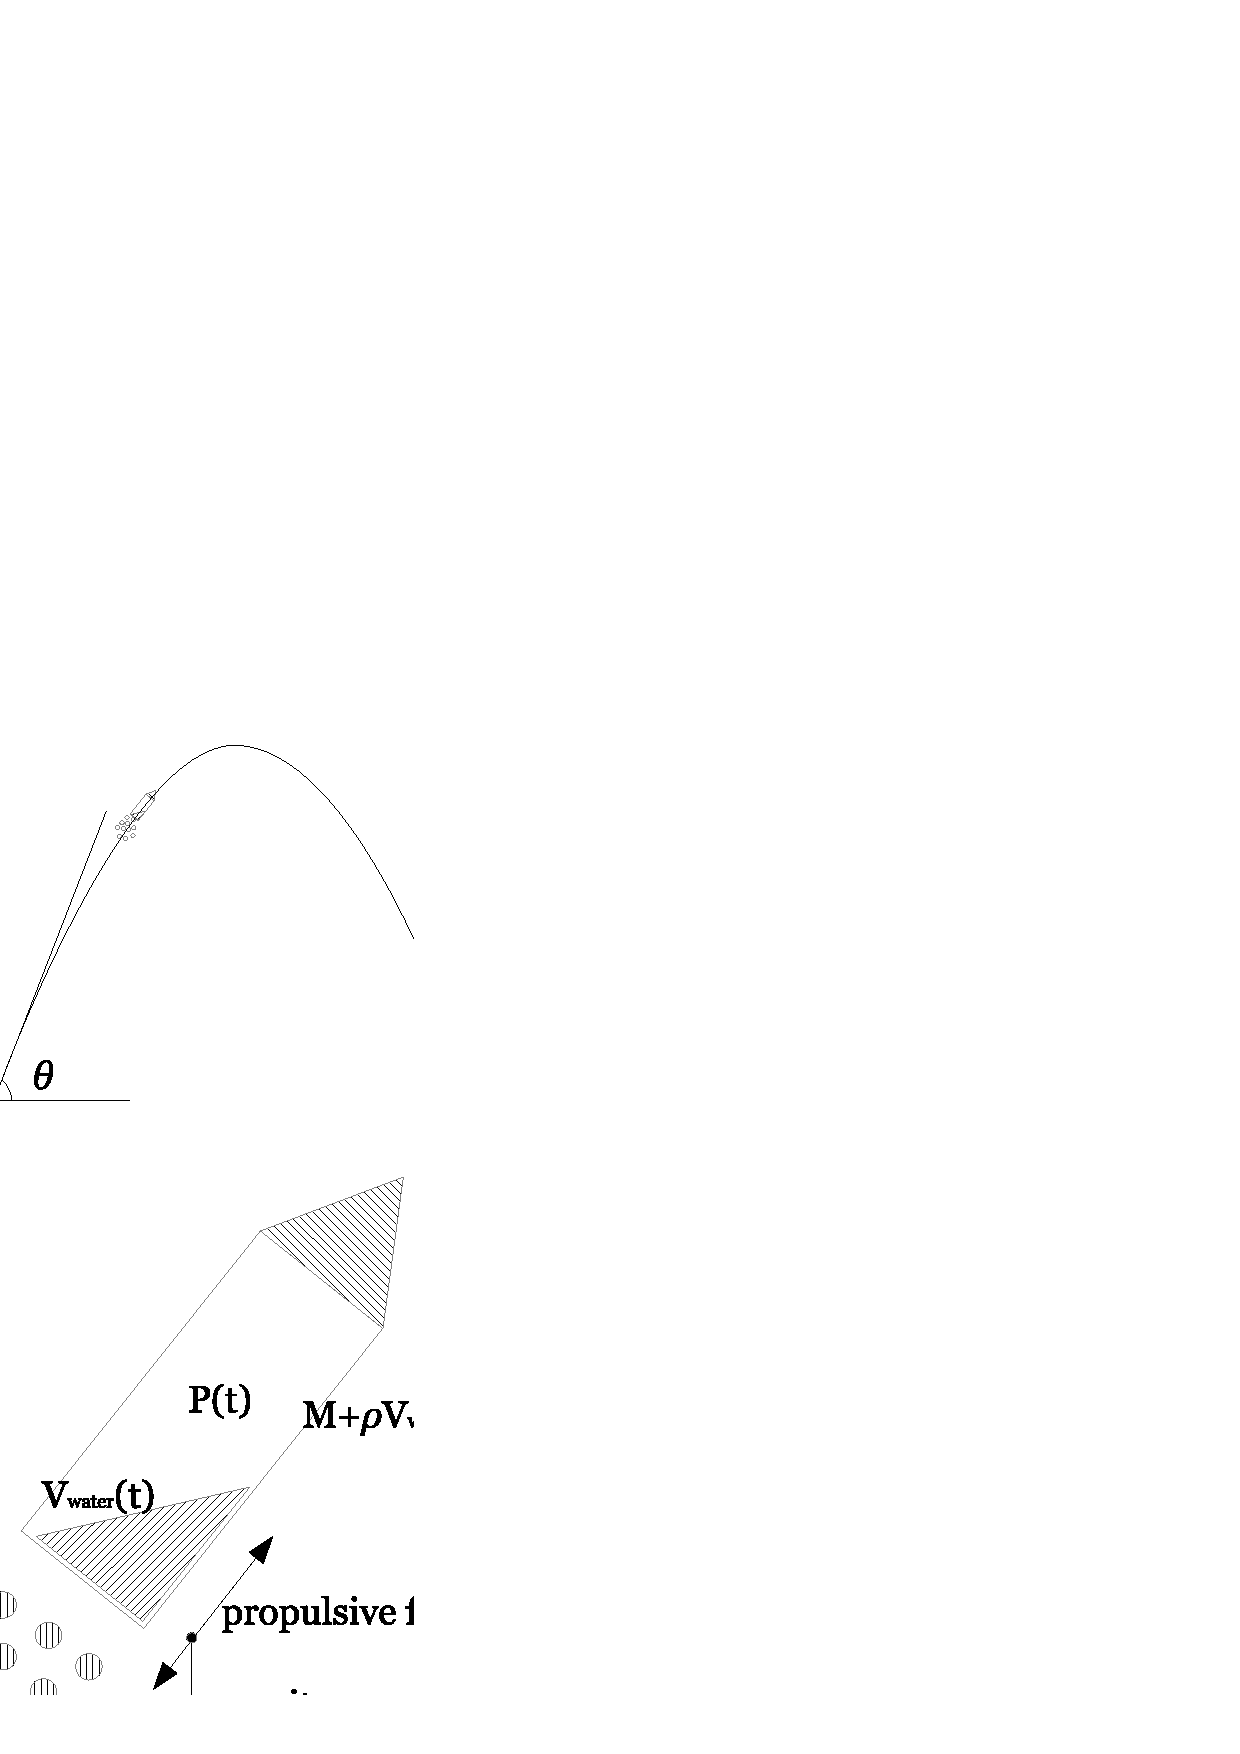
\includegraphics[bb=0mm 0mm 100.0mm 170.0mm, scale=0.35, type=pdf]{img/problem1.pdf}
	% http://atsites.jp/yoshitoharada/1150_Water-rocket1.jpg
\end{figure}
\end{column}
\end{columns}
\end{frame}

%%%%%%%%%%%%%%%%%%%%%%%%%%%%%%%%%%%%%%%%%%%%%%%%%%%%%%%%%%%%%%%%%%%%%%%%%%%%%%%%%%%%%%%%%%%%%%%%%%%%%%%%%%%%

\begin{frame}{問題2}{耐震}
\begin{columns}[t]
\begin{column}{0.7\textwidth}
\begin{wideitemize}
	\item 今回はお休み。どうしてもこれをやりたい人は言ってください。

\end{wideitemize}

\end{column}
\begin{column}{0.3\textwidth}
\begin{figure}[htbp]
    \centering
    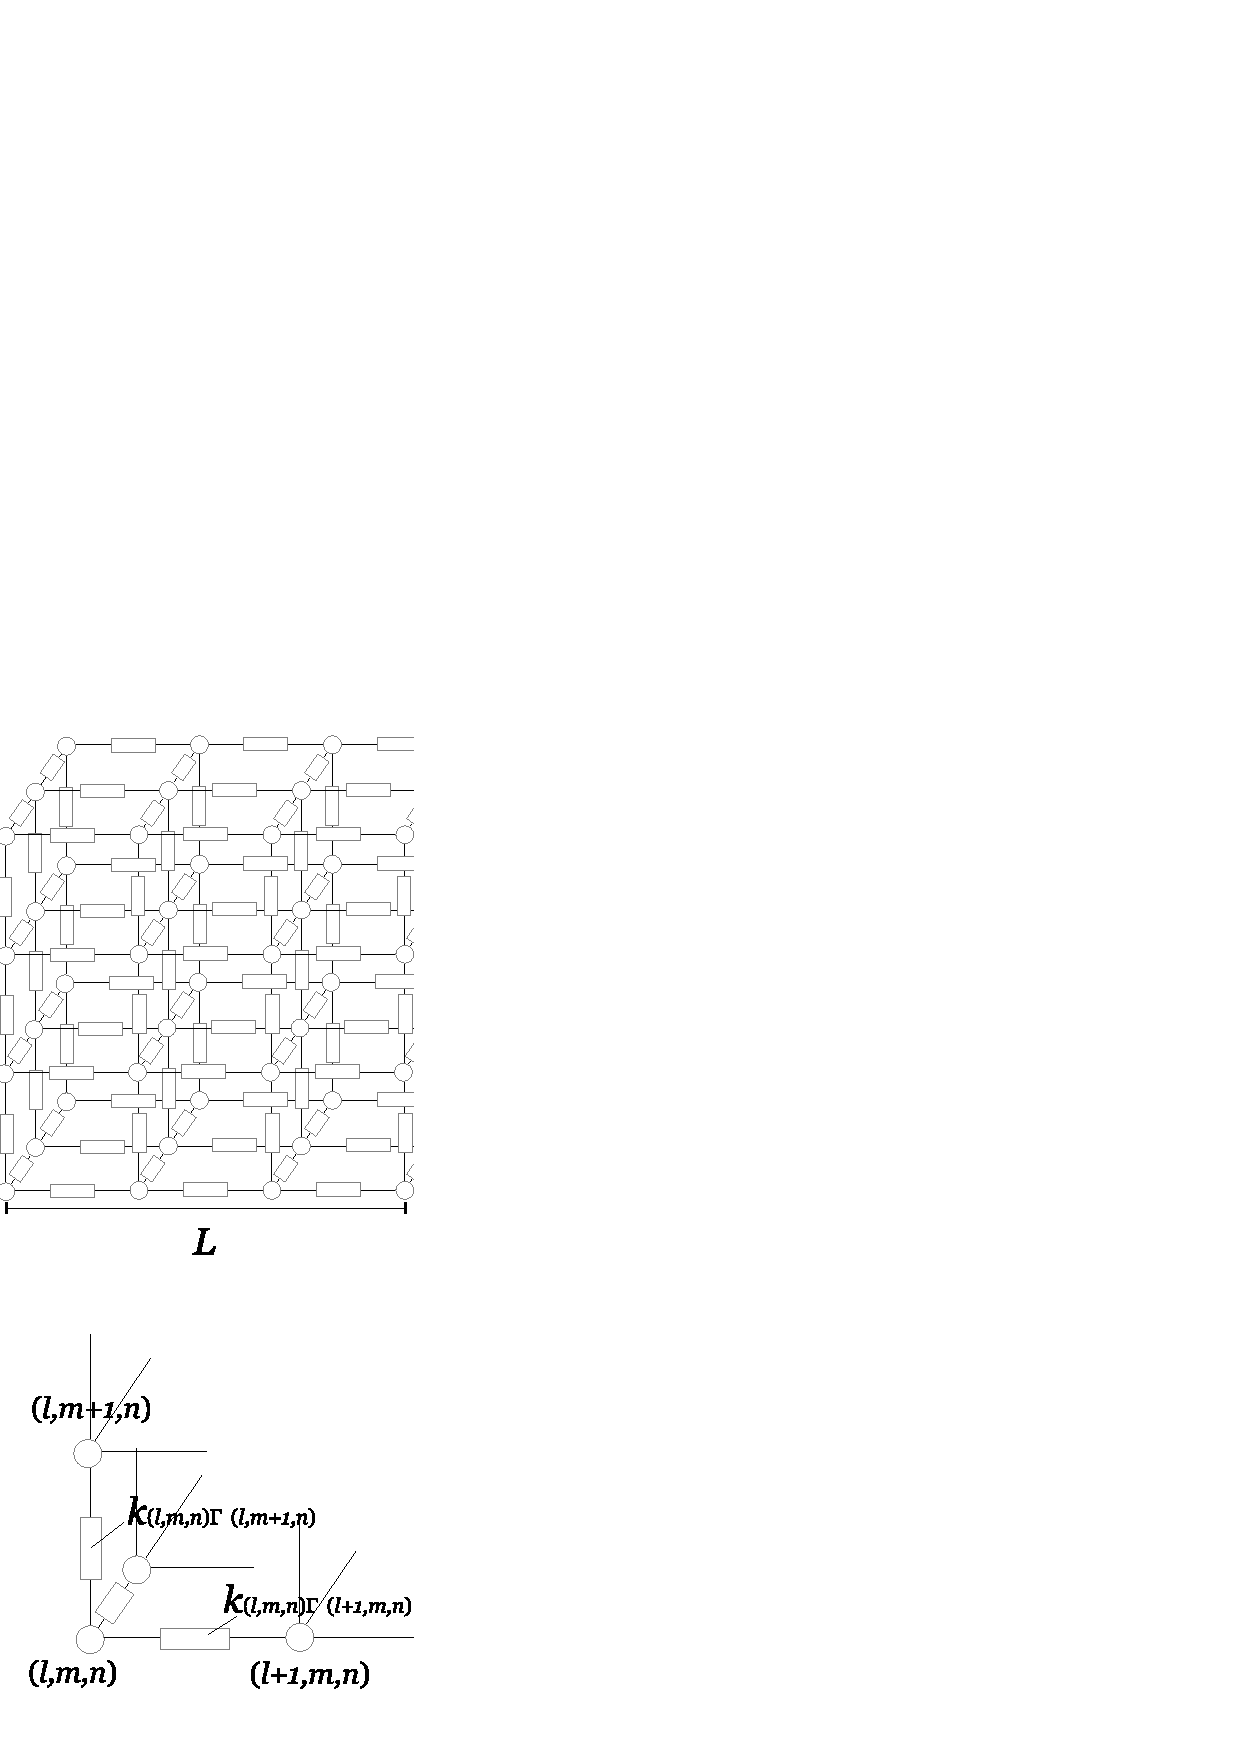
\includegraphics[bb=0mm 0mm 100.0mm 170.0mm, scale=0.35, type=pdf]{img/problem2.pdf}
	% http://ariel-as.eng.hokudai.ac.jp/member/image8.jpg
\end{figure}
\end{column}
\end{columns}
\end{frame}

%%%%%%%%%%%%%%%%%%%%%%%%%%%%%%%%%%%%%%%%%%%%%%%%%%%%%%%%%%%%%%%%%%%%%%%%%%%%%%%%%%%%%%%%%%%%%%%%%%%%%%%%%%%%

\begin{frame}{問題3}{探査衛星とスイングバイ}
\begin{columns}[t]
\begin{column}{0.7\textwidth}
\begin{wideitemize}
	\item 太陽系外に探査機を打ち出したい。打ち上げ日時と位置を求めよ。
	\begin{wideitemize2}
		\item (ボイジャーの打ち上げられた)1977年中に打ち上げる
		\item 太陽の重力場を脱出できる運動エネルギーが得られればよい
		\item 地上発射時の初速は14.5km/sで、地球を黄道面で切った時の断面円周上のどこから打ち上げても良い
		\item 探査機の重さは750kg。ロケットからの分離は考えない
		\item 惑星(太陽~土星まで)は太陽を中心に円軌道を描き、全て同一平面上で運動するとする
		\item 地球の自転の影響を無視して地上から垂直に打ち上げたとする
	\end{wideitemize2}
\end{wideitemize}

\end{column}
\begin{column}{0.3\textwidth}
\begin{figure}[htbp]
    \centering
    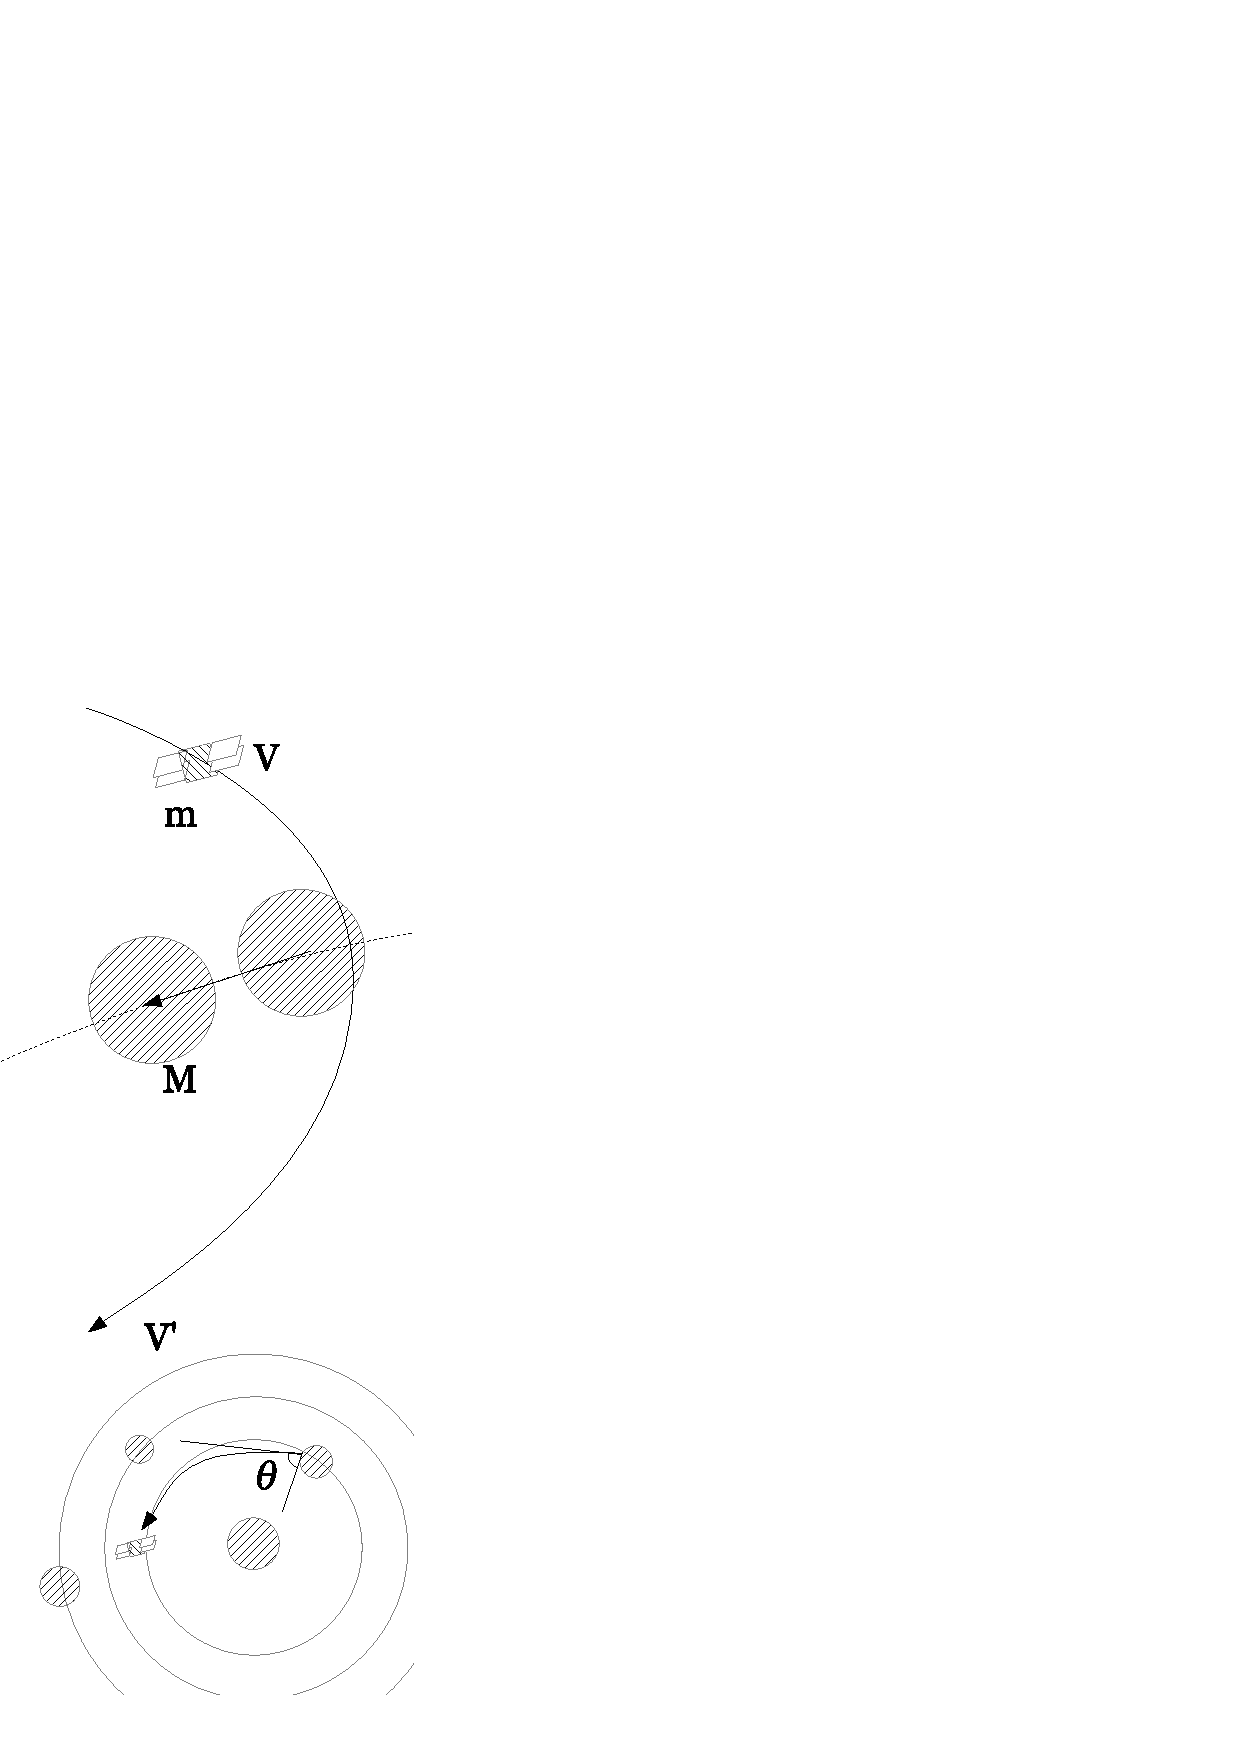
\includegraphics[bb=0mm 0mm 100.0mm 170.0mm, scale=0.35, type=pdf]{img/problem3.pdf}
\end{figure}
\end{column}
\end{columns}
\end{frame}

%%%%%%%%%%%%%%%%%%%%%%%%%%%%%%%%%%%%%%%%%%%%%%%%%%%%%%%%%%%%%%%%%%%%%%%%%%%%%%%%%%%%%%%%%%%%%%%%%%%%%%%%%%%%

% 問題
\begin{frame}{問題4}{空間消音}
\begin{columns}[t]
\begin{column}{0.7\textwidth}
\begin{wideitemize}
	\item 救急車のサイレン音打消しをモデルとして、空間の消音をしたい。消音スピーカーから各々どのような波を出せばよいか
	\begin{wideitemize2}
		\item 幅(x軸)$1.6m$、長さ(y軸)$3.6m$、高さ(z軸)$2m$の大きさの直方体を考え、上面端に$(0, 0, 0)$座標を置く
		\item 960Hzで振幅1の正弦波を出すサイレンが$(0.8,1.8,0)$の位置にある
		\item 消音スピーカーは、高さ$1.6m$、壁面から$0.2m$離れた位置に4つ置く
		\item $(0.6, 2.0, 2.0)$、$(1.0, 2.0, 2.0)$、$(1.0, 2.4, 2.0)$、$(0.6, 2.4, 2.0)$を底面とし、高さが$0.4m$の立方体の空間でエネルギーを最小化する
		\item 標準大気圧で、乾燥しており、温度は25度とする。
	\end{wideitemize2}

\end{wideitemize}

\end{column}
\begin{column}{0.3\textwidth}
\begin{figure}[htbp]
    \centering
    \includegraphics[bb=0mm 0mm 100.0mm 170.0mm, scale=0.35, type=pdf]{img/problem4+.pdf}
\end{figure}
\end{column}
\end{columns}
\end{frame}

%%%%%%%%%%%%%%%%%%%%%%%%%%%%%%%%%%%%%%%%%%%%%%%%%%%%%%%%%%%%%%%%%%%%%%%%%%%%%%%%%%%%%%%%%%%%%%%%%%%%%%%%%%%%

\begin{frame}{問題5}{翼}
\begin{columns}[t]
\begin{column}{0.7\textwidth}
\begin{wideitemize}
	\item 理論的な二次元翼の代表である、ジェコフスキー翼の迎え角と揚力の関係を求めたい
	\begin{wideitemize2}
		\item 気圧は標準大気圧で、気温は25度で湿度はなく、無風である
		\item 空気は粘性流体だが、非圧縮性流体を仮定する
		\item 音速に比べて小さい速度で飛行する(資料と比較できる速度がよい)
		\item 翼長は、資料と比較できるものにする
	\end{wideitemize2}
\end{wideitemize}

\end{column}
\begin{column}{0.3\textwidth}
\begin{figure}[htbp]
    \centering
    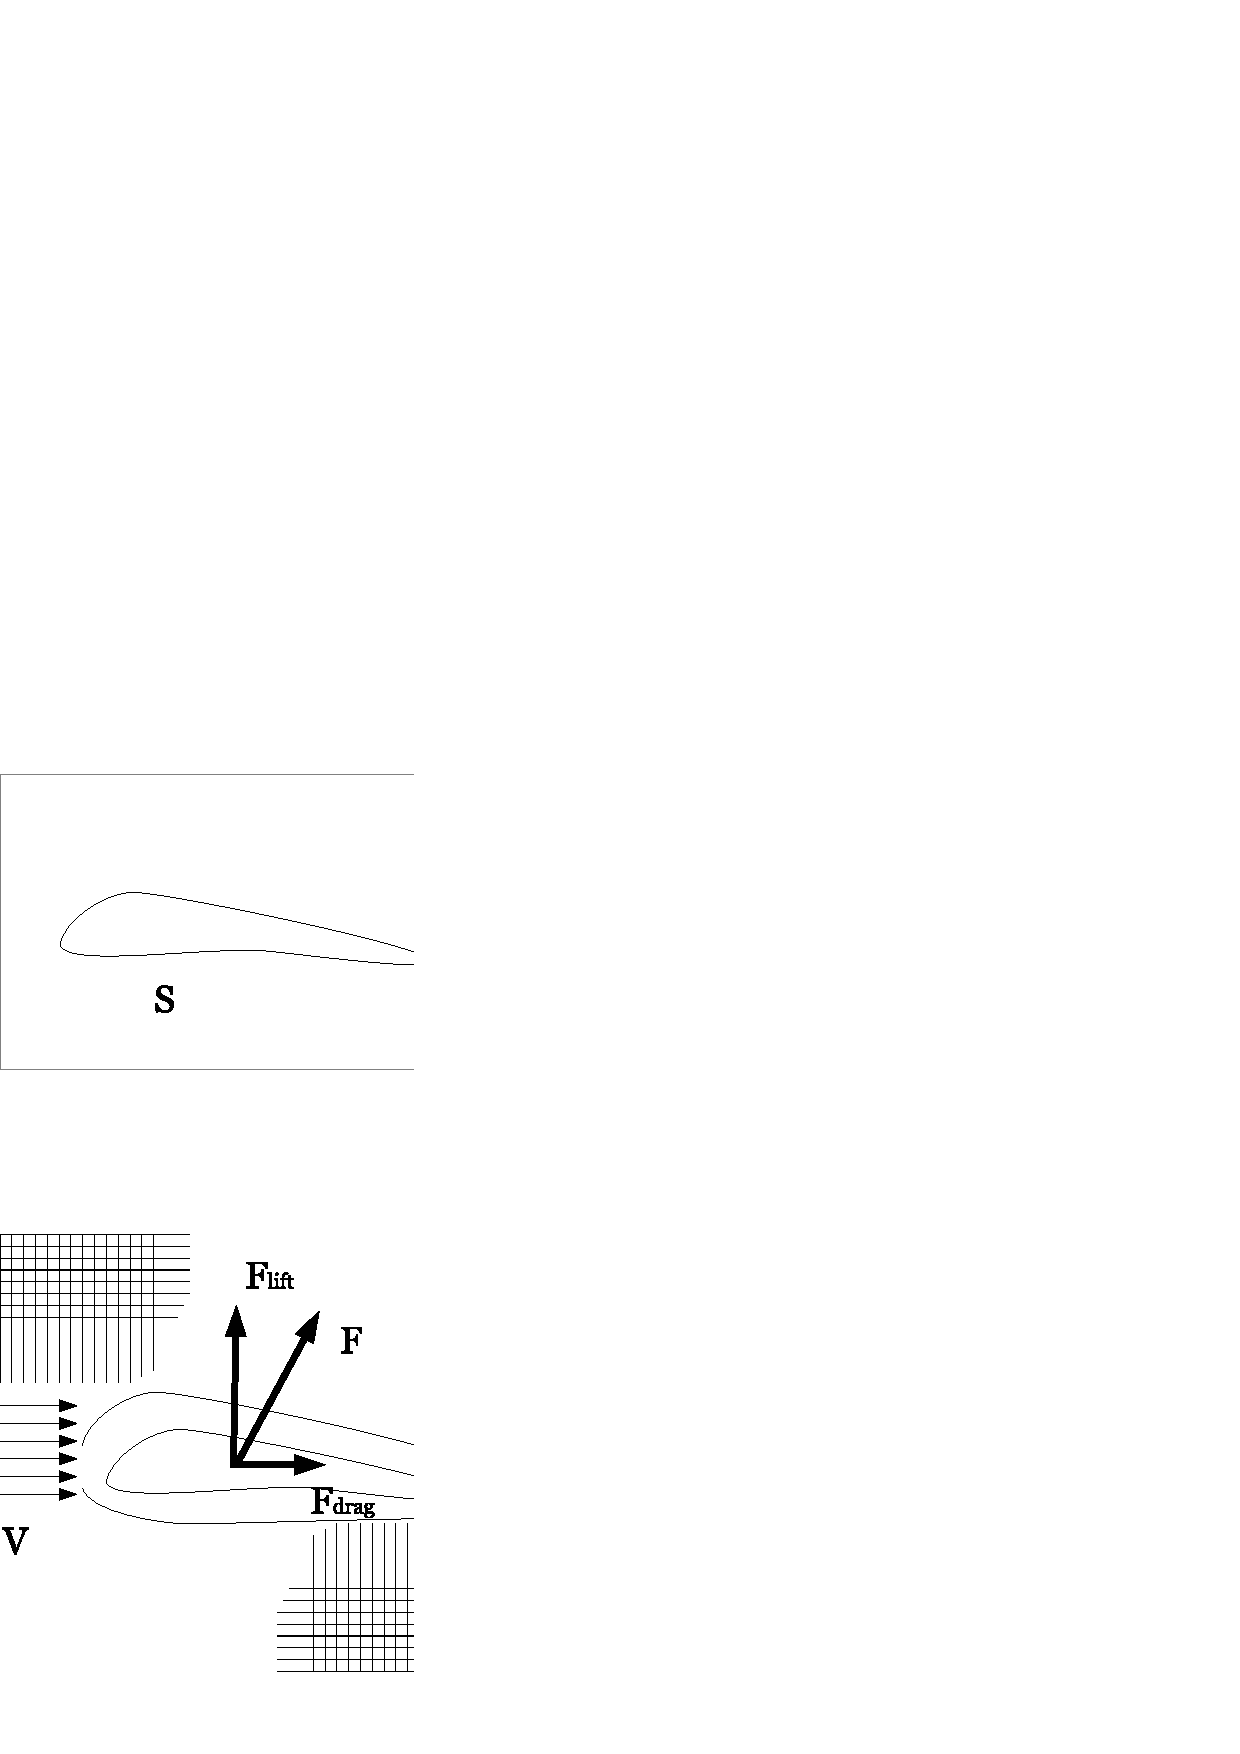
\includegraphics[bb=0mm 0mm 100.0mm 170.0mm, scale=0.35, type=pdf]{img/problem5.pdf}
\end{figure}
\end{column}
\end{columns}
\end{frame}

%%%%%%%%%%%%%%%%%%%%%%%%%%%%%%%%%%%%%%%%%%%%%%%%%%%%%%%%%%%%%%%%%%%%%%%%%%%%%%%%%%%%%%%%%%%%%%%%%%%%%%%%%%%%

\begin{frame}{問題全体を見て}
\begin{wideitemize}
\item 解析的に解くのは難しいものばかり
\item どの問題も一定以上は難しい
\begin{wideitemize2}
	\item 解くべき方程式を立てる、各種係数を探してくる
	\item 最適なパラメータを見つけ出す方法を考える
	\item プログラムに落とし込む
	\item プログラムが正しく動くか(誤差が許容範囲か)確認する
	\item 計算に時間がかかるなら、高速化する
\end{wideitemize2}
\item どれもやりがいがあります
\end{wideitemize}
\end{frame}

\begin{frame}{家でやりたい場合}
\begin{wideitemize}
\item 家でも試してみたいけど、Python入れるのが面倒な人に。
\begin{wideitemize2}
	\item この講義の復習がしたい
	\item 別の講義の課題で使いたい
	\item 趣味でシミュレーション書きたい
\end{wideitemize2}
\item インストール不要で、ダブルクリックで起動できる便利なPython
\item 普段使っているであろうWindows用
\item ここから→\url{http://bit.ly/1EwpGYt}
\begin{wideitemize2}
	\item 不具合があれば教えてください
\end{wideitemize2}
\end{wideitemize}
\end{frame}
% https://drive.google.com/file/d/0B7uRla-1FXs6YUVxRE43NUpmVG8/view?usp=sharing

\end{document}

